\documentclass[addpoints, 12pt]{exam}%, answers]
\usepackage[utf8]{inputenc}
\usepackage[T1]{fontenc}

\usepackage{lmodern}
\usepackage{arydshln}
\usepackage[margin=2cm]{geometry}

\usepackage{enumitem}

\usepackage{amsmath, amsthm, amsfonts, amssymb}
\usepackage{graphicx}
\usepackage{tikz}
\usetikzlibrary{arrows,calc,patterns}
\usepackage{pgfplots}
\pgfplotsset{compat=newest}
\usepackage{url}
\usepackage{multicol}
\usepackage{thmtools}

\usepackage{caption}
\usepackage{subcaption}

\usepackage{pifont}

% MATH commands
\newcommand{\bC}{\mathbb{C}}
\newcommand{\bR}{\mathbb{R}}
\newcommand{\bN}{\mathbb{N}}
\newcommand{\bZ}{\mathbb{Z}}
\newcommand{\bT}{\mathbb{T}}
\newcommand{\bD}{\mathbb{D}}

\newcommand{\cL}{\mathcal{L}}
\newcommand{\cM}{\mathcal{M}}
\newcommand{\cP}{\mathcal{P}}
\newcommand{\cH}{\mathcal{H}}
\newcommand{\cB}{\mathcal{B}}
\newcommand{\cK}{\mathcal{K}}
\newcommand{\cJ}{\mathcal{J}}
\newcommand{\cU}{\mathcal{U}}
\newcommand{\cO}{\mathcal{O}}
\newcommand{\cA}{\mathcal{A}}
\newcommand{\cC}{\mathcal{C}}
\newcommand{\cF}{\mathcal{F}}

\newcommand{\fK}{\mathfrak{K}}
\newcommand{\fM}{\mathfrak{M}}

\newcommand{\ga}{\left\langle}
\newcommand{\da}{\right\rangle}
\newcommand{\oa}{\left\lbrace}
\newcommand{\fa}{\right\rbrace}
\newcommand{\oc}{\left[}
\newcommand{\fc}{\right]}
\newcommand{\op}{\left(}
\newcommand{\fp}{\right)}

\newcommand{\ra}{\rightarrow}
\newcommand{\Ra}{\Rightarrow}

\renewcommand{\Re}{\mathrm{Re}\,}
\renewcommand{\Im}{\mathrm{Im}\,}
\newcommand{\Arg}{\mathrm{Arg}\,}
\newcommand{\Arctan}{\mathrm{Arctan}\,}
\newcommand{\sech}{\mathrm{sech}\,}
\newcommand{\csch}{\mathrm{csch}\,}
\newcommand{\Log}{\mathrm{Log}\,}
\newcommand{\cis}{\mathrm{cis}\,}

\newcommand{\ran}{\mathrm{ran}\,}
\newcommand{\bi}{\mathbf{i}}
\newcommand{\Sp}{\mathrm{span}\,}
\newcommand{\Inv}{\mathrm{Inv}\,}
\newcommand\smallO{
  \mathchoice
    {{\scriptstyle\mathcal{O}}}% \displaystyle
    {{\scriptstyle\mathcal{O}}}% \textstyle
    {{\scriptscriptstyle\mathcal{O}}}% \scriptstyle
    {\scalebox{.7}{$\scriptscriptstyle\mathcal{O}$}}%\scriptscriptstyle
  }
\newcommand{\HOL}{\mathrm{Hol}}
\newcommand{\cl}{\mathrm{clos}}
\newcommand{\ve}{\varepsilon}

\DeclareMathOperator{\dom}{dom}

%%%%%% Définitions Theorems and al.
%\declaretheoremstyle[preheadhook = {\vskip0.2cm}, mdframed = {linewidth = 2pt, backgroundcolor = yellow}]{myThmstyle}
%\declaretheoremstyle[preheadhook = {\vskip0.2cm}, postfoothook = {\vskip0.2cm}, mdframed = {linewidth = 1.5pt, backgroundcolor=green}]{myDefstyle}
%\declaretheoremstyle[bodyfont = \normalfont , spaceabove = 0.1cm , spacebelow = 0.25cm, qed = $\blacktriangle$]{myRemstyle}

%\declaretheorem[ style = myThmstyle, name=Th\'eor\`eme]{theorem}
%\declaretheorem[style =myThmstyle, name=Proposition]{proposition}
%\declaretheorem[style = myThmstyle, name = Corollaire]{corollary}
%\declaretheorem[style = myThmstyle, name = Lemme]{lemma}
%\declaretheorem[style = myThmstyle, name = Conjecture]{conjecture}

%\declaretheorem[style = myDefstyle, name = D\'efinition]{definition}

%\declaretheorem[style = myRemstyle, name = Remarque]{remark}
%\declaretheorem[style = myRemstyle, name = Remarques]{remarks}

\newtheorem{theorem}{Théorème}
\newtheorem{corollary}{Corollaire}
\newtheorem{lemma}{Lemme}
\newtheorem{proposition}{Proposition}
\newtheorem{conjecture}{Conjecture}

\theoremstyle{definition}

\newtheorem{definition}{Définition}[section]
\newtheorem{example}{Exemple}[section]
\newtheorem{remark}{\textcolor{red}{Remarque}}[section]
\newtheorem{exer}{\textbf{Exercice}}[section]


\tikzstyle{myboxT} = [draw=black, fill=black!0,line width = 1pt,
    rectangle, rounded corners = 0pt, inner sep=8pt, inner ysep=8pt]

\begin{document}
	\noindent \hrulefill \\
	MATH-241 \hfill Created by Pierre-O. Paris{\'e}\\
	Worksheet 04 \hfill Fall 2022\\\vspace*{-0.7cm}
	
	\noindent\hrulefill
	
\vspace*{0.5cm}

\noindent\makebox[\textwidth]{\textbf{Last name:}\enspace \hrulefill}
\makebox[\textwidth]{\textbf{First name:}\enspace\hrulefill}
\makebox[\textwidth]{\textbf{Section:}\enspace\hrulefill}

\vspace*{0.25cm}
\begin{center}
\gradetable[h][questions]
\end{center}
\vspace*{0.25cm}

{\bf Instructions:} You must answer all the questions below and give your solutions to the TA at the end of the recitation. Write your solutions directly on the worksheet. Late worksheet will not be accepted.

\qformat{\rule{0.3\textwidth}{.4pt} \begin{large}{\textsc{Question}} \thequestion \end{large} \hspace*{0.2cm} \hrulefill \hspace*{0.1cm} \textbf{(\totalpoints\hspace*{0.1cm} pts)}}

\vspace*{0.5cm}

\begin{questions}

\question

Let $f(x) = x^2 + x$. 

	\begin{parts}
	\part[8]
	Using the definition of the derivative with the limit, find the slope of the tangent line to the graph of $f(x)$ at the point $(1, 2)$.
	\begin{solution}
	{\color{red}
	The slope of the tangent line is given by $f'(1)$. Therefore, using the definition, we have
		\begin{align*}
		f' (1) = \lim_{h \ra 0} \frac{f (1 + h) - f(1)}{h} &= \lim_{h \ra 0} \frac{(1 + h)^2 + (1 + h) - 2}{h} \\
		&= \lim_{h \ra 0} \frac{1 + 2h + h^2 + 1 + h - 2}{h} \\
		&= \lim_{h \ra 0} \frac{3h + h^2}{h} \\
		&= \lim_{h \ra 0} 3 + h \\
		& = 3 .
		\end{align*}
	The slope of the tangent line is therefore $3$.}
	\end{solution}
	
	\part[2]
	Find the equation of the tangent line to the graph of $f(x)$ at the point $(1, 2)$.
	\begin{solution}
	{\color{red}
	The equation of the tangent line is given by
		\begin{align*}
		y - f(1) = f'(1) (x - 1) .
		\end{align*}
	We have $f(1) = 2$ and $f'(1) = 3$. Therefore, we get
		\begin{align*}
		y - 2 = 3 (x - 1) .
		\end{align*}
	The equation of the tangent line is $y = 3x - 1$.}
	\end{solution}
	\end{parts}
	
\newpage

\phantom{2}

\newpage

\question

State if the derivative of the given function $f(x)$ exists at the given number $a$. Explain why the derivative doesn't exist.

	\begin{parts}
	\part[5]
	$f(x) = |x - 1|$ and $a = 1$.
	\begin{solution}
	{\color{red}
	We can plot the graph of the function $f$. We obtain
	
		\begin{center}
		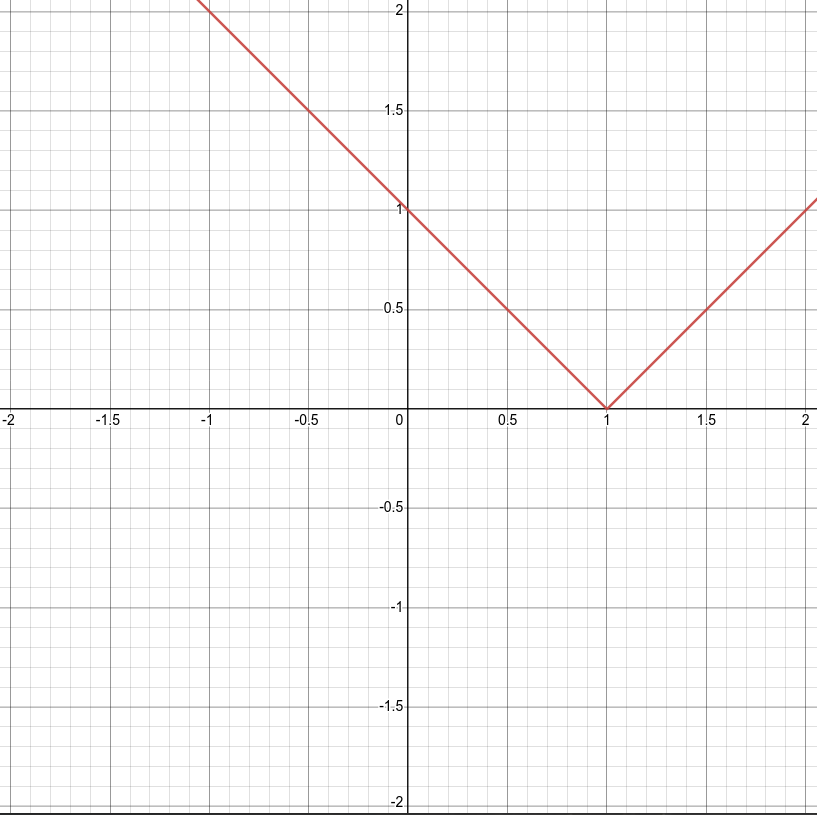
\includegraphics[scale=0.25]{fig_1.png}
		\end{center}
	
	We see that at $a = 1$, we have a break point and therefore the derivative from the left is different from the derivative from the right.
	
	If you use the limit definition of the derivative, then we can show that $f'(1)$ doesn't exist. We first have
		\begin{align*}
		\lim_{h \ra 0^-} \frac{f (1 + h) - f(1)}{h} = \lim_{h \ra 0^-} \frac{-h}{h} = -1 .
		\end{align*}
	We also have
		\begin{align*}
		\lim_{h \ra 0^+} \frac{f (1 + h) - f(1)}{h} = \lim_{h \ra 0^+} \frac{h}{h} = 1 .
		\end{align*}
	We see that the limit from the left is not the same as the limit from the right. Therefore, the derivative of $f$ at $a = 1$ doesn't exist because the limit of the difference quotient doesn't exist.
		}
	\end{solution}
	
	\part[5]
	$ f(x) = \left\{ \begin{matrix} 0 & \text{, if } x = 0 \\ 1/x^2 & \text{, if } x \neq 0 \end{matrix} \right.$ and $a = 0$.
	\begin{solution}
	{\color{red}
	We first have
		\begin{align*}
		\lim_{h \ra 0^-} \frac{f (h) - f(0)}{h} = \lim_{h \ra 0^-} \frac{1}{h^3} = -\infty
		\end{align*}
	The derivative therefore can't exist because we have an infinite limit.}
	\end{solution}
	
	\end{parts}

\newpage

\phantom{2}

\end{questions}

\end{document}